\begin{frame}[noframenumbering]
	\centering
	\huge Performance Results \\ Predictive approach (PA-SPS)
\end{frame}

\begin{frame}{Performance Results : Predictive approach (PA-SPS)}	
	\centering

	\begin{table}[!ht]
	\begin{tabular}{|l|llll|}
	\hline \begin{tabular}[c]{@{}l@{}}Pred.\\ Model\end{tabular} & \begin{tabular}[c]{@{}l@{}}Saved\\ Resources\end{tabular} & \begin{tabular}[c]{@{}l@{}}Throughput\\ Degradation\end{tabular} & \begin{tabular}[c]{@{}l@{}}Diff. Proc.\\ Events\end{tabular} & \begin{tabular}[c]{@{}l@{}}Latency\\ (ms)\end{tabular} \\ \hline \hline
	\textbf{ANN}   & \textbf{0.475} & \textbf{0.070} & \textbf{1.000}      & \textbf{355.490}   \\ \hline
	FFT   & 0.519 & 0.189 & 1.000      & 1023.380 \\ \hline
	LR    & 0.533 & 0.195 & 1.000      & 663.030  \\ \hline
	RF    & 0.538 & 0.227 & 0.996      & 583.921   \\ \hline
	Basic & 0.560 & 0.325 & 1.000      & 1295.490  \\ \hline
	\end{tabular}
	\end{table}
	
	\begin{itemize}
		\item ANN has a low latency and is more stable, but use more resource
		\item Trade-off : Resource vs Performance
	\end{itemize}
\end{frame}

%\begin{frame}{Performance Results}
%	\begin{columns}
%    \begin{column}{0.5\textwidth}
%	    \begin{figure}
%		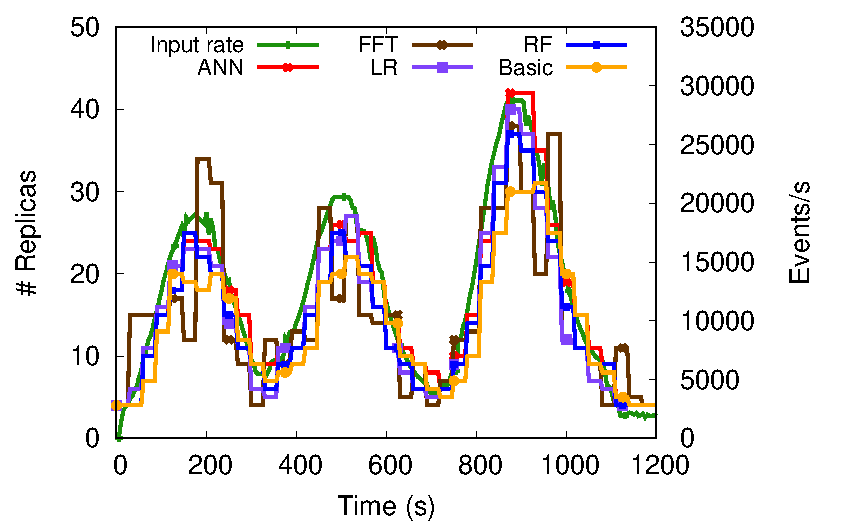
\includegraphics[width=1\textwidth]{images/exp/predictive/TwitterLinear-Models-Replicas.pdf}
%        \caption{Total number of replicas.}
%		\end{figure}
%	\end{column}
%    \begin{column}{0.5\textwidth}
%    	\begin{figure}
%		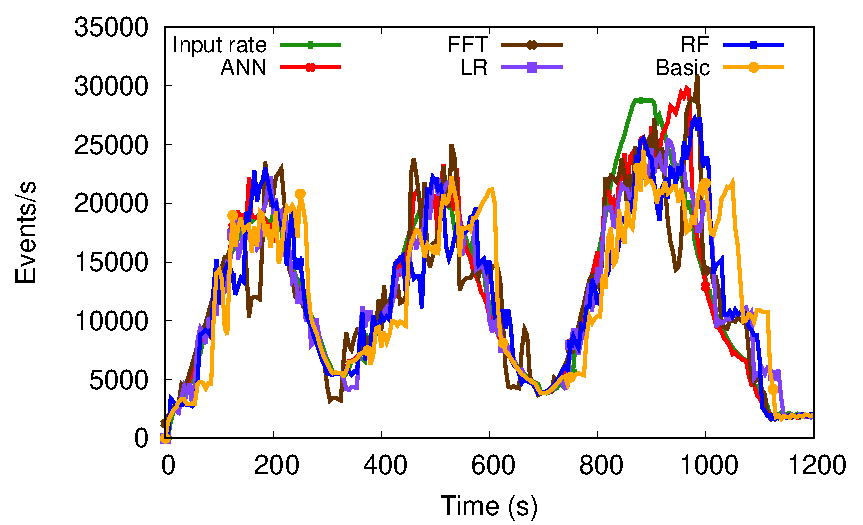
\includegraphics[width=1\textwidth]{images/exp/predictive/TwitterLinear-Models-Throughput.pdf}
%        \caption{Throughput.}
%		\end{figure}
%	\end{column}
%	\end{columns}
%	
%	\begin{center}
%	    Comparison of different models
%	\end{center}
%\end{frame}

\begin{frame}{Performance Results : Predictive approach (PA-SPS)}
	Comparison between PA-SPS and DABS
	\begin{itemize}
		\item PA-SPS : 
		\begin{itemize}
			\item Uses ANN as a predictor model
		\end{itemize}
		\item DABS :
		\begin{itemize}
		 	\item An extension of Storm 
		 	\item Uses a predictor model based on regressions
		\end{itemize}
	\end{itemize}
\end{frame}

\begin{frame}{Performance Results : Predictive approach (PA-SPS)}
	\begin{columns}
    \begin{column}{0.55\textwidth}
    	\centering
	    \begin{figure}
		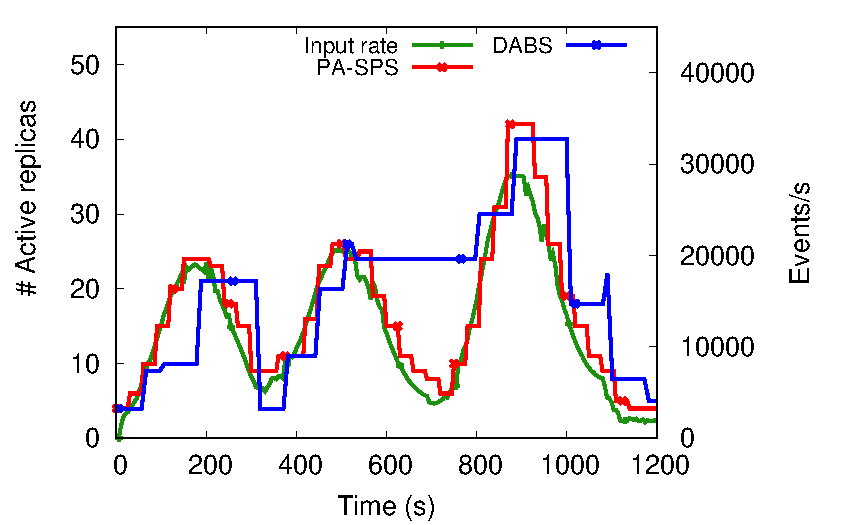
\includegraphics[width=1\textwidth]{images/exp/predictive/TwitterLinear-RW-Replicas.pdf}
		\end{figure}
	\end{column}
    \begin{column}{0.55\textwidth}
    	\centering
    	\begin{figure}
		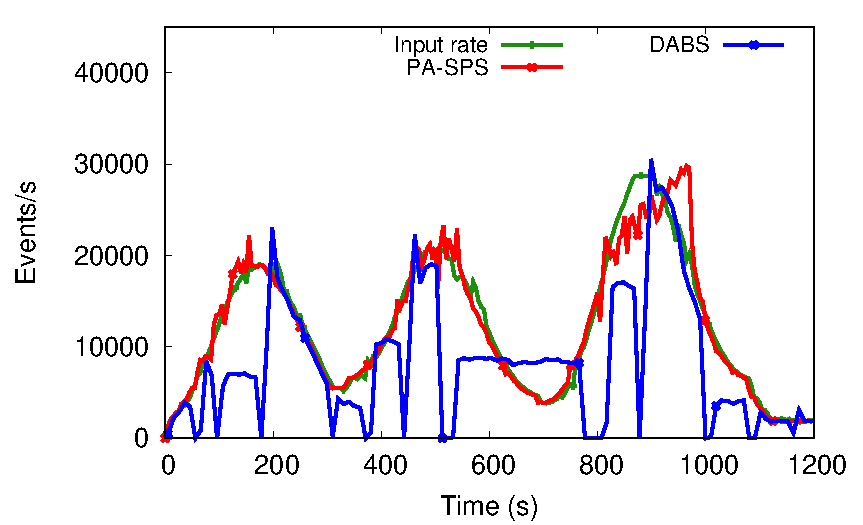
\includegraphics[width=1\textwidth]{images/exp/predictive/TwitterLinear-RW-Throughput.pdf}
		\end{figure}
	\end{column}
	\end{columns}
	
	\begin{itemize}
		\item DABS restarts many times the application
		\item PA-SPS is more stable
	\end{itemize}
\end{frame}

\begin{frame}{Performance Results : Predictive approach (PA-SPS)}
	\centering
	\begin{table}[!ht]
        \begin{tabular}{|l|llll|}
            \hline
          \begin{tabular}[c]{@{}l@{}}Adaptive\\ SPS\end{tabular}  & \begin{tabular}[c]{@{}l@{}}Saved\\ Resources\end{tabular} & \begin{tabular}[c]{@{}l@{}}Throughput\\ Degradation\end{tabular} & \begin{tabular}[c]{@{}l@{}}Diff. Processed\\ Events\end{tabular} & \begin{tabular}[c]{@{}l@{}}Latency\\ (ms)\end{tabular} \\ \hline \hline
            PA-SPS     & 0.475   & 0.071 & 1.000 & 355.490   \\ \hline
            DABS    & 0.3962   & 0.2849 & 0.8283 & 1391.28 \\ \hline
        \end{tabular}
    \end{table}
    \begin{itemize}
    	\item DABS has a less efficient adaptation in contrast to PA-SPS
    \end{itemize}
\end{frame}

%\begin{frame}{Performance Results : Predictive approach (PA-SPS)}	
%	\centering
%	\begin{table}[!ht]
%	\begin{tabular}{|l|llll|}
%	\hline Pred. Model & \begin{tabular}[c]{@{}l@{}}Saved\\ Resources\end{tabular} & \begin{tabular}[c]{@{}l@{}}Throughput\\ Degradation\end{tabular} & \begin{tabular}[c]{@{}l@{}}Diff. Proc.\\ Events\end{tabular} & \begin{tabular}[c]{@{}l@{}}Latency\\ (ms)\end{tabular} \\ \hline \hline
%	ANN PA-SPS   & 0.475 & \textbf{0.070} & \textbf{1.000}      & \textbf{355.490}   \\ \hline
%	LR (DABS) PA-SPS    & \textbf{0.533} & 0.195 & \textbf{1.000}      & 663.030  \\ \hline
%	\end{tabular}
%	\end{table}
%	
%	Metric values
%\end{frame}
